\section{狭义相对论}
对应电动力学课本第七章,占分20分左右。

\begin{question}
    用四维矢量写出电荷守恒定律,
    洛伦兹条件及势方程的相对论的协变形式。
    (需写出第四个分量的具体形式)
\end{question}

\begin{question}
    在反应过程$P+P\rightarrow P+P+\bar P+P$中,设靶粒子静止,计算能使此反应发生的入射粒子的最小动能(即阈能)是多少?
\end{question}

\begin{question}
    两个惯性系$\Sigma $和$\Sigma' $中各放置若干时钟,同一惯性系中的诸时钟同步。
    $\Sigma '$相对于$\Sigma $以速度v沿x轴方向运动。设两系原点相遇时$t_0=t'_0=0$。
    问处于$\Sigma$系中某点$(x,y,z)$处的时钟与$\Sigma' $系中何处的时钟相遇时,指示的时刻相同?读数是多少?
\end{question}

\begin{question}
    (1)由关系式$\mathbf{B}=\nabla \times \mathbf{A}$,$\mathbf{E}=-\nabla \phi-\frac{\partial\mathbf{A}}{\partial t}$,
    引进电磁场张量,并写出此张量的矩阵形式。
    (2)根据张量的变换关系,推导出不同坐标系间的电磁场的变换关系。
\end{question}

\begin{question}
    由洛伦兹变换推出两个事件因果关系不被破坏的条件。由此推出对联系两个因果事件讯号速度的限制。
\end{question}

\begin{question}
    实验证明,带电粒子的电荷与它的运动速度无关,即电荷Q是一个洛仑兹标量,
    由此推出电流密度$\mathbf{J}$和电荷密度$\rho$构成四维矢量$J_\mu(\mathbf{J},i c \rho)$。
\end{question}

\begin{question}
    写出两个电磁场理论和伽利略经典时空观之间的矛盾。
\end{question}

\noindent\textbf{解:}一,牛顿第二定律不是不协变的。

二,电磁波速度不符合伽利略速度叠加公式。

三,S系下的静电场,在运动的S'系下观察除了电磁还有磁场。

\begin{question}
    写出四维速度和四维动量,写出相对论的牛顿第二定律的四维协变形式,并推出四维力的形式。
\end{question}

\begin{question}
    S系为一静止惯性系,S'系以速度v沿x方向运动,有一棍固定在S'系上。
    观察者A和B分别静止于S系和S'系。在t时刻,A对棍进行测量,
    得到棍的长度$l=x_2-x_1=\sqrt{1-\beta^2}l_0$,小于棍的固有长度$l_0$,
    其中$\beta=v/c$。观察者B认为A的测量结果l有错误,为什么?并给出相应的数学推导。
    \begin{figure}[ht]
        \centering
        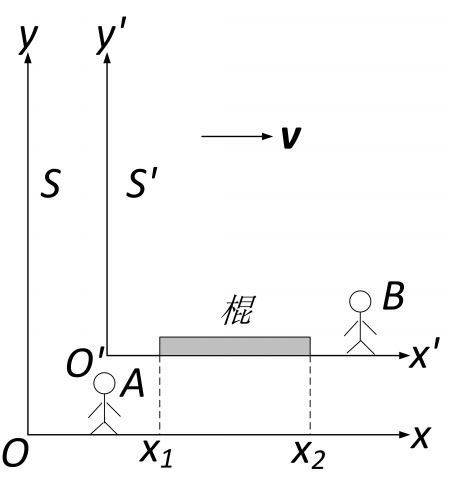
\includegraphics[height=3 cm]{images/q6_1.png}
        \caption{题\thequestion}
    \end{figure}
\end{question}

\begin{question}
    已知$A_\mu(\mathbf{A},i\phi /c)$是一个四维矢量。
    通过电磁场$\mathbf{E}$、$\mathbf{B}$ 与 $\mathbf{A}$、$\phi$ 
    的关系推出电磁场张量$F_{\mu \nu}$,并写出其矩阵表达式。
    利用电磁场张量$F_{\mu \nu}$将麦克斯韦方程组表达成四维形式。
\end{question}

\begin{question}
    在狭义相对论中,每个坐标系中的尺和钟都应相对于该坐标系处于静止状态。
    在同一惯性系内所有的钟都是校准同步的。
    任一物理事件的时空坐标就由该事件发生点的钟和尺的度数来确定。
    试提出一种在同一惯性参照系内钟的校准同步的方法 。
\end{question}

\noindent\textbf{解:}答案不唯一这里提供一种方法,首先量出所有钟到某点的距离。
然后在此点一光速发出信号。收到信号的钟减去信号到达时间。即可同步惯性系中所有的钟。

\begin{question}
    设S'系沿着S系的x轴以速度v运动,两个坐标系的轴互相平行,
    现发生了两个事件1和2,在S'系中测得这两事件的时空坐标为$(x'_1,t'_1)$和$(x'_2,t'_2)$,
    在S系中测得这两事件的时空坐标为$(x_1,t_1)$和$(x_2,t_2)$,
    若在S系这两事件是在不同地点同时发生的,即$t_2=t_1$,$x_2 \neq x_1$那么这两个事件在S'系中是否同时?
    并从洛伦兹变换给出数学推导。
\end{question}

\begin{question}
    写出狭义相对论的基本原理。
\end{question}

\noindent\textbf{解:}第一,相对性原理:在任何惯性参考系中物理现象都按相同的方式发生。
第二光速不变原理。


\begin{question}
    一个质量为$M_0$的静止粒子衰变为静止质量为$m_1$,$m_2$ 的两个粒子,求这两个粒子各自的动能。
\end{question}